\documentclass[11pt,a4paper]{article}

\usepackage{amsfonts}
\usepackage{amssymb}

\usepackage{amsthm}
\usepackage{epsfig}
\usepackage{graphicx}
\usepackage{natbib}		% citet, citep
\usepackage{textcomp}
\usepackage{booktabs}
\usepackage{multirow}
\usepackage{fullpage}
\usepackage{authblk}
\usepackage{url}
\usepackage{color}
\usepackage{tikz}
\usepackage{float}
% \usepackage{xeCJK}
% \setCJKmainfont{TW-Kai} 

% use for game tree
\usepackage{amsmath}
\def\vpay#1#2{\begin{matrix}#1\\#2\end{matrix}}
\usepackage{istgame}

\renewcommand{\baselinestretch}{1.4}

\parskip=5pt
\parindent=20pt
\footnotesep=5mm

\newtheorem{lem}{Lemma}
\newtheorem{prop}{Proposition}
\newtheorem{defn}{Definition}
\newtheorem{cor}{Corollary}
\newtheorem{ass}{Assumption}
\newtheorem{obs}{Observation}
\newenvironment{pf}{\begin{proof}\vspace{-10pt}}{\end{proof}}
% \newtheorem{ques}{Question}
% \newtheorem{rmk}{Remark}
% \newtheorem{note}{Note}
% \newtheorem{eg}{Example}

\newenvironment{enumerateTight}{\begin{enumerate}\vspace{-8pt}}{\end{enumerate}\vspace{-8pt}}
\newenvironment{itemizeTight}{\begin{itemize}\vspace{-8pt}}{\end{itemize}\vspace{-8pt}}
\leftmargini=25pt   % default: 25pt
\leftmarginii=12pt  % default: 22pt

\DeclareMathOperator*{\argmax}{argmax}
\DeclareMathOperator*{\argmin}{argmin}
\setcounter{MaxMatrixCols}{20}

\title{Computer Network and Application (110-1) \\ Homework 2}

\author{Michael Chen (B08705051)}
\date{}

\begin{document}

\maketitle

\section{R5}
The IP address and port number.

\section{R9}
SSl operates at the application layer.\\
If the application developer wants TCP to be enhanced with SSL, he/she has to add the SSL code into the application.

\section{R19}
MX records are used to deliver emails to your address, it'll tell where emails sent to your domain should be routed to.\\
Because a organization can have the same hostname for its web server and mail server, a MX record is used to  to obtain the 
canonical name for the “mail server”, while the CNAME record is used to obrain the canonical name of the web server.

\section{R23}
If a BitTorrent tracker suddenly becomes unavailable, the users can't update their list of peers. The users won't know if 
there's a new peer arriving or a peer just left.\\
Existing users can still find peers with his list of peers and request for data(if no one left). But new users won't be able 
to obtain any data from peers.\\
However, files can still be downloaded, since the user can request it from server directly, just much slower than p2p.

\section{P3}
\begin{enumerate}
    \item The browser checks DNS record caches to find IP address of \texttt{http://yourbusiness.com}
    \item If the browser can't find it in caches, ISP's DNS server would send a DNS query to find IP address
    \item The browser sends an HTTP GET request to the server to request for \texttt{about.html}
    \item The server will handle the request and send an HTTP response
    \item The browser displays the content of \texttt{about.html}
\end{enumerate}

\section{P18}
\subsection{a}
WHOIS database contains records of registeration and IP information of registered domains.

\subsection{b}
\begin{itemize}
    \item Google DNS server
    \item Cloudflare
\end{itemize}
using GoDaddy TW

\subsection{c}
\begin{figure}[H]
    \centering
    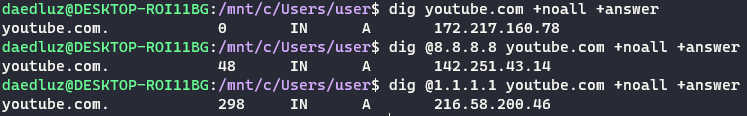
\includegraphics[width=\linewidth]{./img/TypeA.png}
    \caption{Type A}
    \label{Type A}
\end{figure}

\begin{figure}[H]
    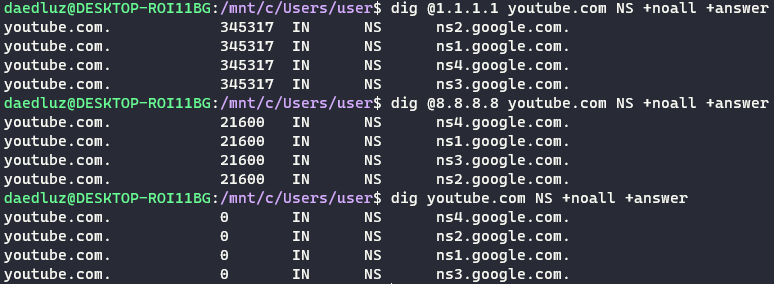
\includegraphics[width=\linewidth]{./img/TypeNS.png}
    \caption{Type NS}
    \label{Type NS}
\end{figure}

\begin{figure}[H]
    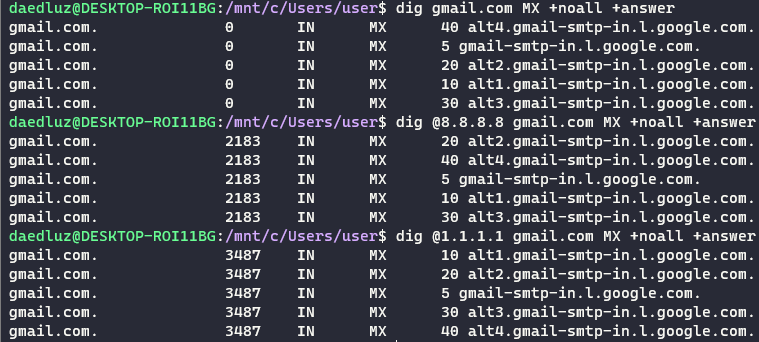
\includegraphics[width=\linewidth]{./img/TypeMX.png}
    \caption{Type MX}
    \label{Type MX}
\end{figure}

\subsection{d}
I searched for www.youtube.com and found various IP.\\
But there's only one IP for www.ntu.edu.tw (140.112.8.116).

\subsection{e}
The range is 140.112.0.0 to 140.112.255.255

\subsection{f}
The attacker can use whois database and nslookup tool to get every IP address of the institution and target those IP 
during his attack.

\subsection{g}
WHOIS database contains registeration and IP informations of domains, if it's not publicly avaliable, it would 
be hard to obtain informations about domains and find out who's responsible for the domain (useful for tracing cybercrimes).

\section{P29}
Yes, you can configure your browser to open multiple simultaneous connections to a website.\\
The advantage is that it can help client to download different data from the same server simultaneously.\\
The disadvantage is that multiple connections causes more network traffic, which may leads to congestion.

\section{P31}
Netflix runs their website on Amazon cloud to handle user login, movie catalog and recommendation etc. They have private CDN 
servers to deliver video content to users. By doing so, Netflix simplifies its CDN design.\\
Netflix replicates content by process it on the Amazon cloud first, then upload it to different CDN servers.

\end{document}